\documentclass{chi-ext}
% Please be sure that you have the dependencies (i.e., additional LaTeX packages) to compile this example.
% See http://personales.upv.es/luileito/chiext/

%% EXAMPLE BEGIN -- HOW TO OVERRIDE THE DEFAULT COPYRIGHT STRIP -- (July 22, 2013 - Paul Baumann)
% \copyrightinfo{Permission to make digital or hard copies of all or part of this work for personal or classroom use is granted without fee provided that copies are not made or distributed for profit or commercial advantage and that copies bear this notice and the full citation on the first page. Copyrights for components of this work owned by others than ACM must be honored. Abstracting with credit is permitted. To copy otherwise, or republish, to post on servers or to redistribute to lists, requires prior specific permission and/or a fee. Request permissions from permissions@acm.org. \\
% {\emph{IHM14}}, 28-31 Octobre, 2014, Lille, France. \\
% Copyright \copyright~2014 ACM ISBN/14/04...\$15.00. \\
% DOI string from ACM form confirmation}
%% EXAMPLE END -- HOW TO OVERRIDE THE DEFAULT COPYRIGHT STRIP -- (July 22, 2013 - Paul Baumann)

\title{IHM \LaTeX\ Ext. Abstracts Template}

\numberofauthors{6}
% Notice how author names are alternately typesetted to appear ordered in 2-column format;
% i.e., the first 4 autors on the first column and the other 4 auhors on the second column.
% Actually, it's up to you to strictly adhere to this author notation.
\author{
  \alignauthor{
  	\textbf{Premier Auteur}\\
  	\affaddr{AuthorCo, Inc.}\\
  	\affaddr{123 Author Ave.}\\
  	\affaddr{Authortown, PA 54321 USA}\\
  	\email{author1@anotherco.com}
  }\alignauthor{
  	\textbf{Quatrième Author}\\
  	\affaddr{AuthorCo, Inc.}\\
  	\affaddr{123 Author Ave.}\\
  	\affaddr{Authortown, PA 54321 USA}\\
  	\email{author5@anotherco.com}
  }
  \vfil
  \alignauthor{
  	\textbf{Deuxième Auteur}\\
  	\affaddr{AuthorCo, Inc.}\\
  	\affaddr{123 Author Ave.}\\
  	\affaddr{Authortown, PA 54321 USA}\\
  	\email{author2@anotherco.com}
  }\alignauthor{
  	\textbf{Cinquième Author}\\
  	\affaddr{AuthorCo, Inc.}\\
  	\affaddr{123 Author Ave.}\\
  	\affaddr{Authortown, PA 54321 USA}\\
  	\email{author6@anotherco.com}
  }
  \vfil
  \alignauthor{
  	\textbf{Troisième Author}\\
  	\affaddr{AuthorCo, Inc.}\\
  	\affaddr{123 Author Ave.}\\
  	\affaddr{Authortown, PA 54321 USA}\\
  	\email{author3@anotherco.com}
  }\alignauthor{
  	\textbf{Sixième Author}\\
  	\affaddr{AuthorCo, Inc.}\\
  	\affaddr{123 Author Ave.}\\
  	\affaddr{Authortown, PA 54321 USA}\\
  	\email{author7@anotherco.com}
  }
}

% Paper metadata (use plain text, for PDF inclusion and later re-using, if desired)
\def\plaintitle{CHI LaTeX Extended Abstracts Template}
\def\plainauthor{Luis A. Leiva}
\def\plainkeywords{Guides, instructions, author's kit, conference publications}
\def\plaingeneralterms{Documentation, Standardization}

\hypersetup{
  % Your metadata go here
  pdftitle={\plaintitle},
  pdfauthor={\plainauthor},  
  pdfkeywords={\plainkeywords},
  pdfsubject={\plaingeneralterms},
  % Quick access to color overriding:
  %citecolor=black,
  %linkcolor=black,
  %menucolor=black,
  %urlcolor=black,
}

\usepackage{graphicx}   % for EPS use the graphics package instead
\usepackage{balance}    % useful for balancing the last columns
\usepackage{bibspacing} % save vertical space in references
%\usepackage{hyperref}
%\hypersetup{colorlinks=false}

%\widowpenalty=10000
%\clubpenalty=10000

\begin{document}

\maketitle

\begin{abstract}
Dans cet exemple nous décrivons les règles de formatage pour les Travaux en Cours (TeC) IHM, ainsi que des conseils de rédaction.
%Ne changez pas la taille des pages ou les paramètres des pages.
Veuillez lire ce document, même si vous avez déjà soumis : il peut y avoir des différences.
\end{abstract}

\keywords{\plainkeywords}
\textcolor{red}{Champs requis dans la version finale}

\category{H.5.m}{Information interfaces and presentation (e.g., HCI)}{Miscellaneous}. 
%See \cite{ACMCCS} 
Voir : \url{http://www.acm.org/about/class/1998/} 
pour une description du ACM Classification system.
\textcolor{red}{Champs requis dans la version finale}

\terms{\plaingeneralterms}
\textcolor{red}{Champs requis dans la version finale}


% =============================================================================
\section{Introduction}
% =============================================================================
Ce format est à utiliser pour les TeC, qui sont publiés dans les actes étendus. 
Ces articles doivent conserver une apparence consistante et de qualité. 
Nous vous demandons donc de suivre ces règles de formatage simples.
Dans l'idée, vous devez formatter votre papier de la même façon que ce document.
La façon la plus simple est de télécharger le template sur le site web de la conférence et de remplacer le contenu par votre propre matériel.

% =============================================================================
\section{Copyright}
% =============================================================================

Les auteurs conservent le copyright pour les articles publiés en TeC.
Ces articles ne sont pas considérés comme des publications d'archive, mais sont tout de même publiés sur la Digital Library ACM.
Le fait que vous conserviez le copyright signifie que vous êtes libre de réutiliser votre matériel comme vous l'entendez, y compris soumettre un article à propos de ce matériel à une autre conférence ou journal.
Les auteurs donnent à l'ACM une permission sans réseve de publier les soumissions acceptées dans les actes étendus d'IHM sans considération ou rémunération supplémentaire.

% =============================================================================
\section{Formatage du texte}
% =============================================================================
Veuillez utiliser une police Verdana de 8.5 points, ou toute autre police sans sérif ayant une apparence proche de Verdana, utilisée dans ce document.
La police Arial en 9 points est un substitut raisonnable car elle a une taille similaire.
Veuillez n'utiliser une police à sérif ou de taille différente que pour des cas spéciaux, tels que mettre en avant du code source.
De plus voici un exemple de note de bas de page.\footnote{Utilisez les notes de bas de page avec parcimonie, et que si nécessaire.}
Comme précisé dans la note de bas de page, les notes de bas de page doivent être rarement utilisées.

\subsection{Langue, style, et contenu}
% -----------------------------------------------------------------------------
La langue officielle d'IHM est le français. Les soumissions en anglais sont autorisées, cependant en français comme en anglais la qualité de rédaction est un critère d'évaluation. Nous rappelons que la \href{http://www.sigchi.org/conferences/organizing-a-sigchi-sponsored-conference}{politique de l'ACM} autorise la publication d'une traduction en anglais d'un article écrit dans une langue différente.
Les règles de typographie doivent être adaptées à la langue de l'article.
Pour vous assurer d'être compréhensible, veuillez suivre ces conseils :

\begin{itemize}\compresslist
\item 	
Utilisez un style direct.
Utilisez des structures de phrase simples.
Essayez d'éviter des phrases longues avec des structures compliquées.
Utilisez les point-virgule avec précaution.
\item 	
Utilisez un vocabulaire courant et usuel (ex. : utilisez le mot « inhabituel » plutôt que « ésotérique »).
\item 	
Définissez ou expliquez brièvement chaque terme technique.
La terminologie courante dans votre discipline peut être différente de celle dans d'autres disciplines.
\item 	
Détaillez tous les acronymes la première fois que vous les utilisez dans votre texte.
Par exemple « Interaction Homme-Machine (IHM) »
\item 	
Expliquez les références locales (ex. : tout le monde ne connait pas tous les noms de ville dans une région particulière).
\item 	
Expliquez les commentaires d'initiés.
Assurez vous que tout le monde comprend toutes les références à ce que vous ne décrivez pas (ex. : ne supposez pas que tout le monde a déjà utilisé un Mac ou une application particulière).
\item 	
Expliquez le langage familier ou les jeux de mots.
Comprendre une expression telle que « poisson d'avril » nécessite des connaissance culturelles françaises.
L'humour et l'ironie sont difficiles à traduire.
\item 	
Utilisez des formes non ambigües selon la culture, tel que les dates, heures, monnaies et nombres (ex. : « 1-5-14 » ou « 5/1/14 » qui peuvent vouloir dire 5 janvier ou 1er mai, ou « sept heures » peut vouloir dire 7h ou 19h.).
\item 	
Faites attention avec l'utilisation de pronoms spécifiques au genre (il, elle) et autres mots dépendants du genre (ex. : homme-mois).
Utilisez un langage inclusif (ex. : il ou elle, ils ou elles, personne-mois) qui sont indépendants du genre.
Si nécessaire, vous pouvez utiliser « il » et « elle » en alternant dans vos phrases, de manière à équilibrer les genres. 
\end{itemize}


% =============================================================================
\section{Figures}
% =============================================================================

\marginpar{
\begin{figure}
  \begin{center}
  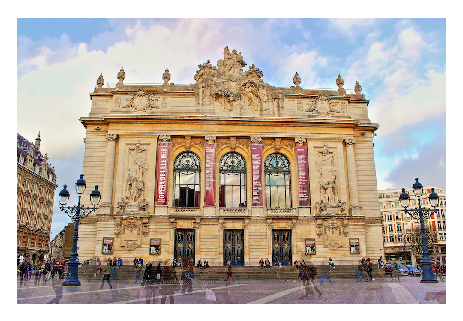
\includegraphics[width=\marginparwidth]{images/lille.eps}
  \caption{Une figure dans la marge.}
  \label{fig:marginparsample}
  \end{center}  
\end{figure}
}

Les exemples dans cette page et les suivantes devraient vous donner une idée de comment les photos et screenshots doivent être placés dans le template. 
Assurez-vous que vos images soient assez grandes pour que les détails soient visibles et clairs.

\begin{figure}
  \centering
  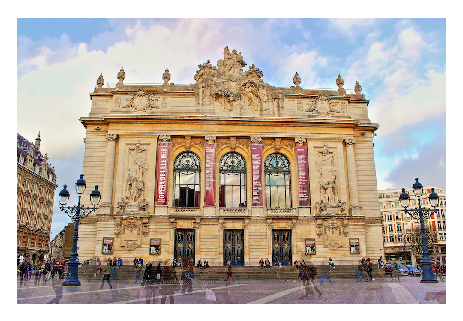
\includegraphics[width=\linewidth]{images/lille.eps}
  \caption{Ajoutez une légende en dessous de chaque image.}
  \label{fig:sample}
\end{figure}

Votre document peut utiliser des figures en couleurs, qui sont comprises dans les limites de pages ; les figures doivent rester lisibles si le document est imprimé en noir et blanc.
Vous pouvez utiliser la commande \LaTeX \texttt{marginpar} pour insérer des figures dans la marge de gauche (voir \autoref{fig:marginparsample}).


% =============================================================================
\section{Références et Citations}
% =============================================================================
Utilisez une liste numérotée à la fin de l'article, par ordre alphabétique du premier auteur, et référencée par des numéros entre crochets~\cite{mbl-ihm-97,coutaz-ihm-97,guiard-jmb-87}
Pour les articles dans des actes de conférences, indiquez le titre du papier et une version abrégée du nom de la conférence (ex. : pour les actes d'IHM 2001, utilisez « Actes d'IHM 2001 »).
N'ajoutez pas le lieu de la conférence ou la date exacte ; ajoutez les numéros de pages si disponibles.
Voyez des exemples de citations à la fin de ce document.

Vos références doivent être du matériel publié et accessible au public.
Les rapports internes peuvent être cités si ils sont aisément accessibles (ex. : vous donnez l'adresse pour obtenir le rapport dans votre citation) et peuvent être obtenus par n'importe quel lecteur pour une somme modique.
Les informations propriétaires ne devraient pas être citées.
Les communications privées doivent être mentionnées dans le texte principal, pas référencées (ex. : [Georges Abitbol, personal communication]).

% =============================================================================
\section{Produire et tester le fichier PDF}
% =============================================================================
Nous vous recommandons de produire une version PDF de votre soumission bien avant la date butoir.
En plus de vérifier que vous pouvez produire un PDF, vous devrez vérifier que (a) la longueur du fichier reste dans les limites fixéers par la catégorie visée, (b) le fichier PDF n'excède pas 4 Mo, et (c) le fichier peut être lu et imprimé avec Adobe Acrobat Reader.
Testez votre PDF en le visionnant et l'imprimant avec le même logiciel que nous quand nous le recevrons, Adobe Acrobat Reader 10.
Ce logiciel est très répandu et gratuit~\cite{Acrobat10}.  

% =============================================================================
\section{Dummy text}
% =============================================================================
Lorem ipsum dolor sit amet, consectetur adipiscing elit. Duis ut eros semper lectus vehicula elementum. Vestibulum ante ipsum primis in faucibus orci luctus et ultrices posuere cubilia Curae; Aliquam quis mi sapien. Suspendisse potenti. Mauris ultrices euismod velit sed dictum. Nullam auctor, nulla tincidunt dapibus suscipit, velit leo convallis metus, vel commodo libero erat in dolor. In laoreet porttitor ligula, porta blandit lectus consequat quis. 

Nam ut eros dui. Mauris volutpat elit metus, euismod pellentesque purus. In hac habitasse platea dictumst. Nullam consectetur lacinia interdum. Sed nec blandit nisi. Proin in nulla purus, sit amet iaculis tortor. Ut dapibus pellentesque nulla in interdum. Nunc at velit felis. Curabitur euismod neque eu orci varius in pharetra sem interdum. Morbi in mauris ac risus iaculis dapibus id in magna. Class aptent taciti sociosqu ad litora torquent per conubia nostra, per inceptos himenaeos.

Aliquam consectetur quam sed odio varius vitae rhoncus urna fermentum. Phasellus viverra diam non justo porttitor varius. Integer ultrices accumsan lectus eget mollis. Nulla et leo sit amet nunc ornare rutrum sit amet ac dui. Cras vehicula accumsan purus nec fermentum. Mauris viverra condimentum metus, ut posuere quam laoreet nec. Phasellus massa tellus, ullamcorper nec porta sed, aliquet vitae nulla. Phasellus non tortor mauris. Cras ullamcorper egestas erat, vel rutrum elit viverra a. Donec in nisl ut est facilisis blandit. Quisque congue accumsan risus, ut venenatis magna vulputate vel. Nam commodo sapien vel mauris adipiscing nec dictum quam congue. Phasellus tempor vestibulum nisl quis blandit. Nullam condimentum auctor nibh, quis elementum libero tristique.



\section{Remerciements}
Nous remercions toutes les personnes qui ont successivement modifié ce format. Nous nous sommes basés sur la version distribuée pour CHI 2013, et qui est à ce jour la version officielle \url{http://personales.upv.es/luileito/chiext/}.

\section{Format des références}
Les références doivent utiliser la même taille de police que le reste du texte.
% REFERENCES FORMAT
% References must be the same font size as other body text.

\balance
\bibliographystyle{acm-sigchi}
\bibliography{ref}

\end{document}